\documentclass[10pt,letterpaper]{article}
\usepackage[latin1]{inputenc}
\usepackage{amsmath}
\usepackage{amsfonts}
\usepackage{amssymb}
\usepackage{tikz}
\usepackage{graphicx}
\usepackage{caption}
\usepackage{subcaption}
\usepackage[top=1in,bottom=1in,right=1in,left=1in]{geometry}
\begin{document}
\interfootnotelinepenalty=10000
\raggedbottom
\begin{center}
Moneyball with Pig and Hive \\
Russ Lankenau \\ 
rlankenau@maprtech.com
\end{center}

The provided data contains various information about Major League Baseball between 1921 and 2011.  The data is freely available on the web from retrosheet.org\footnote{http://www.retrosheet.org/game.htm}.  The majority of the data is in the form of event records, i.e. plays.  Each play describes an event that occurs when a batter steps up to the plate.  This could be an out, a hit, or some other event such as a runner stealing a base.  In addition, there are other types of data such as team rosters, game information, player lists, team lists, and reconstructed data for games where no clear record exists.

\begin{table}[h]
\begin{tabular}{rl}
info & Information about a single game (e.g. time of day, weather, location)\\
start & A starting player, including name, ID, position, home/away, and batting order\\
sub & A player substituted in during play\\
play & A single event during a game\\
com & A comment inserted by the recorder\\
id & The game ID, consisting of year, month, day, and game number for the day\\
version & The file version\\
data & Additional data about a player (e.g. number of errors during the game)\\ 
\end{tabular}
\caption{Record Types}
\end{table}

The records are comma-separated, and are intermixed within the event files.  Each event file contains the home games for a single team for a single year. American League teams are listed in .EVA files, and National League teams are listed in .EVN files.    

\begin{figure}[h]
\begin{align}
&start,\overbrace{grudm001}^\text{Player ID},\overbrace{"Mark Grudzielanek"}^\text{Player Name},\overbrace{0}^\text{Home(1) or Away(0)},\overbrace{1}^\text{Batting Order},\overbrace{6}^\text{Position} \nonumber \\
&play,\overbrace{1,0}^\text{Inning},\overbrace{aaroh101}^\text{Player ID},\overbrace{12}^\text{Count},\overbrace{BF1CX}^\text{Pitches},\overbrace{\underbrace{S}_\text{Play Type}\underbrace{7}_\text{Fielder(s)}/\underbrace{L7S}_\text{Description}.\underbrace{3-H;1-2}_\text{Runner movement}}^\text{Play} \nonumber
\end{align}
\caption{Sample Records}
\end{figure}

The provided sample code\footnote{https://github.com/rlankenau/mapr-moneyball} extracts one very basic metric, a count of plays for each player, grouped by ball location and result.  Using the sample as a guide, can we extract other interesting data from this data set?

\begin{itemize}
\item What is the relationship between player names and IDs? (e.g. one-to-one?)
\item Which player has the most career RBIs?
\item Can we tell which players' performance drops off most in later innings?
\item Which players are the most consistent between home games and away games?
\item
\item
\end{itemize}

\begin{center}
\begin{figure}
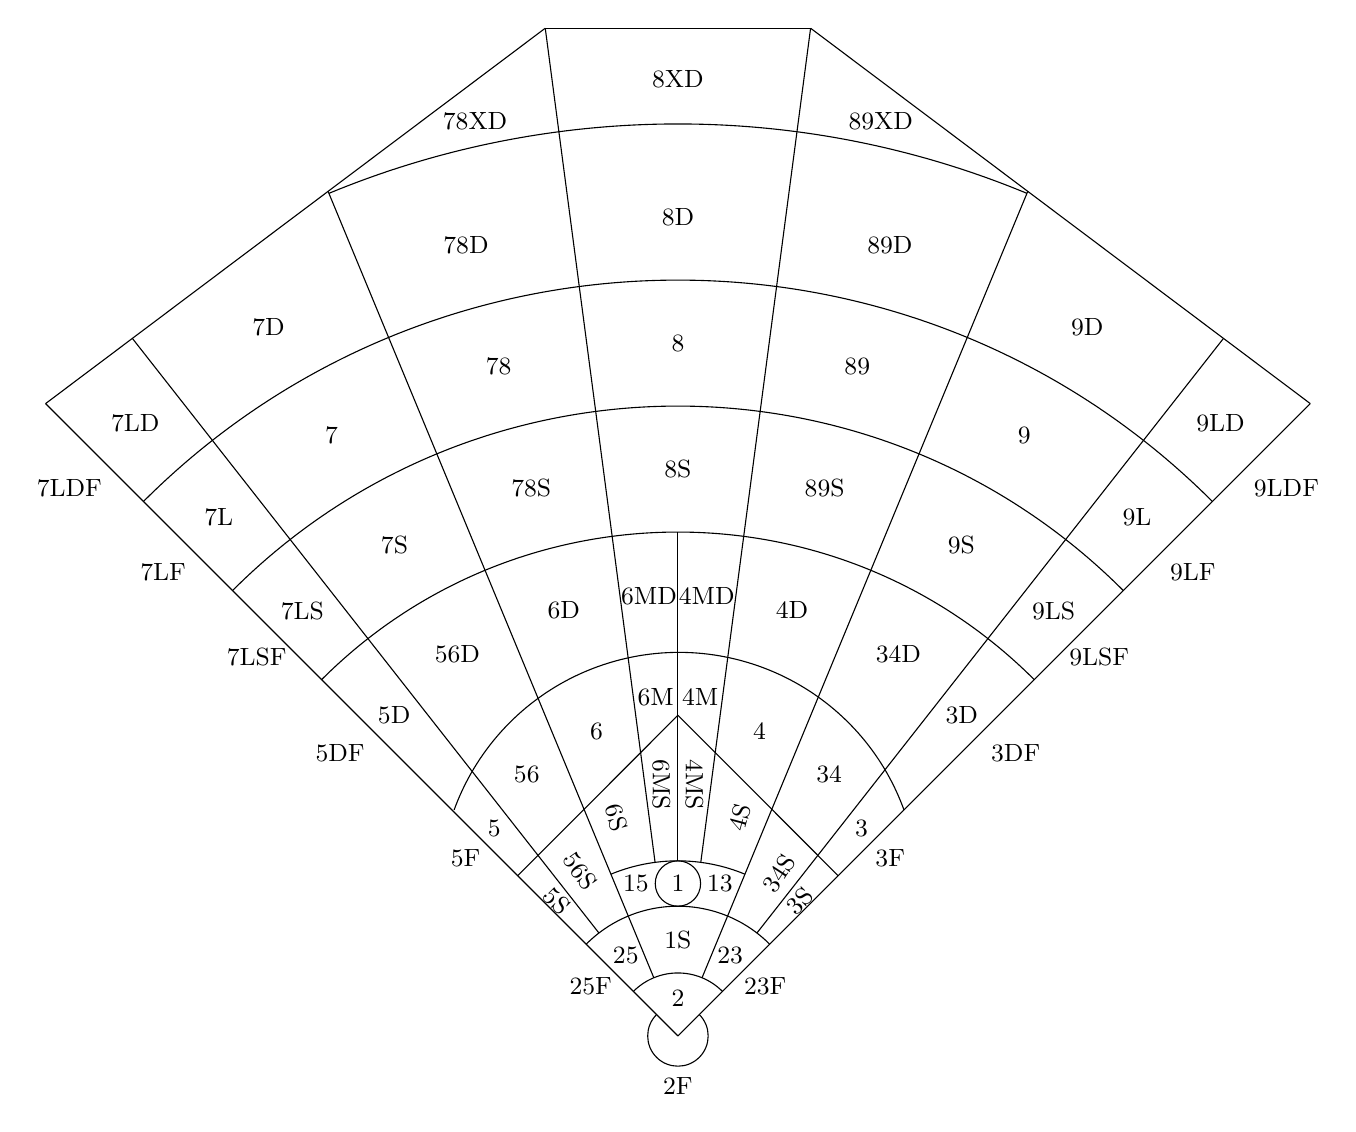
\begin{tikzpicture}[scale=.032]
\tikzstyle{every node}=[font=\small]

\coordinate (HomePlate) at (0,0);
\coordinate (LeftFieldFoul) at (-251,251);
\coordinate (RightFieldFoul) at (251,251);
\coordinate (CenterField) at (0,400);
\coordinate (CenterFieldLeft) at (-52.6610, 400);
\coordinate (CenterFieldRight) at (52.6610, 400);
\coordinate (Pitcher) at (0,60.5);
\coordinate (ThirdBase) at (-63.6, 63.6);
\coordinate (FirstBase) at (63.6, 63.6);
\coordinate (SecondBase) at (0,127.3);


\draw (HomePlate) -- (LeftFieldFoul);
\draw (HomePlate) -- (RightFieldFoul);
\draw (LeftFieldFoul) -- (CenterFieldLeft);
\draw (RightFieldFoul) -- (CenterFieldRight);
\draw (CenterFieldLeft) -- (CenterFieldRight);

\draw (ThirdBase) -- (SecondBase);
\draw (FirstBase) -- (SecondBase);

\draw (Pitcher) circle (9) node{1};
\draw (Pitcher) node[left=7pt]{15};
\draw (Pitcher) node[right=7pt]{13};
\draw (-8.4866,8.4866) arc (135:405:12);
\draw (0,38) node {1S};
\draw ({38*cos(123)},{38*sin(123)}) node {25};
\draw ({38*cos(57)},{38*sin(57)}) node {23};
\draw (0,15) node {2};
\draw (0,-20) node {2F};
\draw (89.7167,89.7167) arc (20:160:95);
\draw (36.416,36.416) arc (45:135:51.5);
\draw (26.5965,64.2096) arc (67.5:112.5:69.5);
\draw (17.68,17.68) arc (45:135:25);

\draw (0,69.5) -- (0,200);
\draw (9.5671,23.0970) -- (138.862,335.242);
\draw (-9.5671, 23.0970) -- (-138.862,335.242);
\draw (-9.0716, 68.9054) -- (CenterFieldLeft);
\draw (9.0716, 68.9054) -- (CenterFieldRight);
\draw ({51.5*cos(52.5)},{51.5*sin(52.5)}) -- (216.5460, 276.8831);
\draw ({51.5*cos(127.5)},{51.5*sin(127.5)}) -- (-216.5460, 276.8831);
\draw ({200*cos(45)},{200*sin(45)}) arc (45:135:200);
\draw ({175*cos(93.75)},{175*sin(93.75)}) node {6MD};
\draw ({175*cos(86.25)},{175*sin(86.25)}) node {4MD};
\draw ({135*cos(93.75)},{135*sin(93.75)}) node {6M};
\draw ({135*cos(86.25)},{135*sin(86.25)}) node {4M};
\draw ({100*cos(93.75)},{100*sin(93.75)}) node[rotate=270] { 6MS};
\draw ({100*cos(86.25)},{100*sin(86.25)}) node[rotate=270] { 4MS};
\draw ({90*cos(105.75)},{90*sin(105.75)}) node[rotate=285] { 6S};
\draw ({90*cos(74.25)},{90*sin(74.25)}) node[rotate=75] { 4S};
\draw ({76*cos(120.75)},{76*sin(120.75)}) node[rotate=305] { 56S};
\draw ({76*cos(58.25)},{76*sin(58.25)}) node[rotate=57] { 34S};
\draw ({72*cos(132)},{72*sin(132)}) node[rotate=315] { 5S};
\draw ({72*cos(48)},{72*sin(48)}) node[rotate=45] { 3S};
\draw (0,225) node {8S};
\draw ({250*cos(45)},{250*sin(45)}) arc (45:135:250);
\draw (0,275) node {8};
\draw ({300*cos(45)},{300*sin(45)}) arc (45:135:300);
\draw (0,325) node {8D};
\draw ({362*cos(67.5)},{362*sin(112.5)}) arc (67.5:112.5:362);
\draw (0,380) node {8XD};
\draw ({125*cos(105)},{125*sin(105)}) node {6};
\draw ({175*cos(105)},{175*sin(105)}) node {6D};
\draw ({225*cos(105)},{225*sin(105)}) node {78S};
\draw ({275*cos(105)},{275*sin(105)}) node {78};
\draw ({325*cos(105)},{325*sin(105)}) node {78D};
\draw ({372*cos(102.5)},{372*sin(102.5)}) node {78XD};
\draw ({125*cos(75)},{125*sin(75)}) node {4};
\draw ({175*cos(75)},{175*sin(75)}) node {4D};
\draw ({225*cos(75)},{225*sin(75)}) node {89S};
\draw ({275*cos(75)},{275*sin(75)}) node {89};
\draw ({325*cos(75)},{325*sin(75)}) node {89D};
\draw ({372*cos(77.5)},{372*sin(77.5)}) node {89XD};
\draw ({120*cos(120)},{120*sin(120)}) node {56};
\draw ({175*cos(120)},{175*sin(120)}) node {56D};
\draw ({225*cos(120)},{225*sin(120)}) node {7S};
\draw ({275*cos(120)},{275*sin(120)}) node {7};
\draw ({325*cos(120)},{325*sin(120)}) node {7D};
\draw ({120*cos(60)},{120*sin(60)}) node {34};
\draw ({175*cos(60)},{175*sin(60)}) node {34D};
\draw ({225*cos(60)},{225*sin(60)}) node {9S};
\draw ({275*cos(60)},{275*sin(60)}) node {9};
\draw ({325*cos(60)},{325*sin(60)}) node {9D};
\draw ({110*cos(48.5)},{110*sin(48.5)}) node {3};
\draw ({170*cos(48.5)},{170*sin(48.5)}) node {3D};
\draw ({225*cos(48.5)},{225*sin(48.5)}) node {9LS};
\draw ({275*cos(48.5)},{275*sin(48.5)}) node {9L};
\draw ({325*cos(48.5)},{325*sin(48.5)}) node {9LD};
\draw ({110*cos(131.5)},{110*sin(131.5)}) node {5};
\draw ({170*cos(131.5)},{170*sin(131.5)}) node {5D};
\draw ({225*cos(131.5)},{225*sin(131.5)}) node {7LS};
\draw ({275*cos(131.5)},{275*sin(131.5)}) node {7L};
\draw ({325*cos(131.5)},{325*sin(131.5)}) node {7LD};
\draw ({325*cos(138)},{325*sin(138)}) node {7LDF};
\draw ({275*cos(138)},{275*sin(138)}) node {7LF};
\draw ({225*cos(138)},{225*sin(138)}) node {7LSF};
\draw ({175*cos(140)},{175*sin(140)}) node {5DF};
\draw ({110*cos(140)},{110*sin(140)}) node {5F};
\draw ({40*cos(150)},{40*sin(150)}) node {25F};
\draw ({325*cos(42)},{325*sin(42)}) node {9LDF};
\draw ({275*cos(42)},{275*sin(42)}) node {9LF};
\draw ({225*cos(42)},{225*sin(42)}) node {9LSF};
\draw ({175*cos(40)},{175*sin(40)}) node {3DF};
\draw ({110*cos(40)},{110*sin(40)}) node {3F};
\draw ({40*cos(30)},{40*sin(30)}) node {23F};
\end{tikzpicture}
\caption{Field Locations}
\end{figure}
\end{center}
\begin{table}
\subfloat[Positions]{
\begin{tabular}{rl}
1 & Catcher\\ 
2 & Pitcher\\ 
3 & First Base\\ 
4 & Second Base\\ 
5 & Third Base\\ 
6 & Shortstop\\ 
7 & Left Field\\ 
8 & Center Field\\ 
9 & Right Field\\
\end{tabular}}
\subfloat[Play Type]{
\begin{tabular}{rl}
(none) & Out \\
S & Single \\
D & Double \\
T & Triple \\
HR & Home Run \\
HP & Hit by pitch \\
W & Walk \\
IW & Int. Walk \\
WP & Wild Pitch \\
\end{tabular}}
\subfloat[Description]{
\begin{tabular}{rl}
G & Ground Ball \\
L & Line Drive \\
P & Pop Fly \\
F & Fly Ball \\
B & Prefix indicating bunt \\
\end{tabular}}
\subfloat[Pitches]{
\begin{tabular}{rl}
C & Called Strike \\
S & Swinging Strike \\
B & Ball \\
F & Foul Ball \\
L & Foul Bunt \\
M & Missed Bunt \\
P\footnotemark & Pitchout\\
I & Int. Ball \\
H & Hit by pitch \\
K & Strike (unknown) \\
U & Unknown \\
n\footnotemark & Pickoff \\
\end{tabular}}
\caption{Play Codes}
\end{table}  
\footnotetext[2]{Rarely, a pitchout will result in a strike or foul ball.  These are recorded as Q and R respectively.}
\footnotetext[3]{n is 1, 2, or 3, corresponding to base thrown to. The base number is preceded by a '+' if the pickoff was thrown by the pitcher.}
\end{document}
